\chapter{Learning a metric for clustering}\label{chap:clustering-metric}
In section \ref{sec:mil-clustering}, a method for learning a representation \( \phi \) was shown. In order to learn the parameters of the representation, a clustering-loss function is required in the form
\[ L_C : \mathcal{P}^M \left( \bar{\mathspace{X}} \right) \to \mathfield{R} \]
In this chapter, several different ways of constructing such a clustering-loss function are explored.

\section{Contrastive predictive coding}
Contrastive predictive coding is a technique first introduced by \cite{oord_representation_2019}. In this section, the original article is first presented, with its application to MIL clustering introduced subsequently.

\subsection{Original article}
\name{Contrastive predictive coding} (also referred to as \name{CPC}) builds the model on the ideas from predictive coding (see \cite{elias_predictive_1955}), a technique from information theory. In predictive coding, a sequence of messages is transmitted. Both the transmitter and the receiver try to predict future messages from all the past ones. Only the difference between the predicted and actual message is then actually transmitted.

CPC is an approach to representing time series by modelling future data from the past. In order to do that, the model learns high-level representations of the data and discards noise in the data. The further in future the model predicts, the less shared information is available and thus the global structure needs to be inferred better.

First, a non-linear encoder \( g_\mathrm{enc} \) is used to map an input sequence of data to their latent representations:
\[ g_\mathrm{enc} : x_t \mapsto z_t \]
Next, an autoregressive model \( g_\mathrm{ar} \) summarizes all latent representations up to a certain point \( t \) and produces a context latent representation:
\[ c_t = g_\mathrm{ar} \left( \left\{ z_i \middle| i \leq t \right\} \right) \]
Modelling \( p_k \left( x_{t + k} \middle| c_t \right) \) directly using a conditional generative model is computationally very expensive, which is the reason why this approach hasn't been chosen. Instead, the density ratio which preserves the mutual information between \( x_{t + k} \) and \( c_t \) has been modelled as follows:
\begin{equation}\label{equa:CPC-model}
  f_k \left( x_{t + k}, c_t \right) \propto \frac{p \left( x_{t + k} \middle| c_t \right)}{p \left( x_{t + k} \right)}
\end{equation}
A log-bilinear model was used:
\[ f_k \left( x_{t + k}, c_t \right) = \mathrm{exp} \left( z_{t + k}^T W_k c_t \right) \]

Both \( g_\mathrm{enc} \) and \( g_\mathrm{ar} \) have been trained to jointly optimize a loss based on the Noise Contrastive Estimation (see \cite{gutmann_noise-contrastive_2010}), which is called \name{InfoNCE} in \cite{oord_representation_2019}. Given a set \( \mathset{X} = \left\{ x_1, \dots, x_N \right\} \) containing one positive sample from \( p \left( x_{t + k} \middle| c_t \right) \) and \( N - 1 \) negative samples from \( p \left( x_{t + k} \right) \), the InfoNCE loss is as follows:
\[ L_N = - \underset{\mathset{X}}{\mathbb{E}} \left[ \log \frac{f_k \left( x_{t + k}, c_t \right)}{\sum_{x_j \in \mathset{X}} f_k \left( x_j, c_t \right)} \right] \]
Optimising \( L_N \) will result in \( f_k \) estimating the density ratio from equation \ref{equa:CPC-model}.

The model is illustrated in figure \ref{fig:CPC-paper-model}.

\begin{figure}[h]
	\centering
	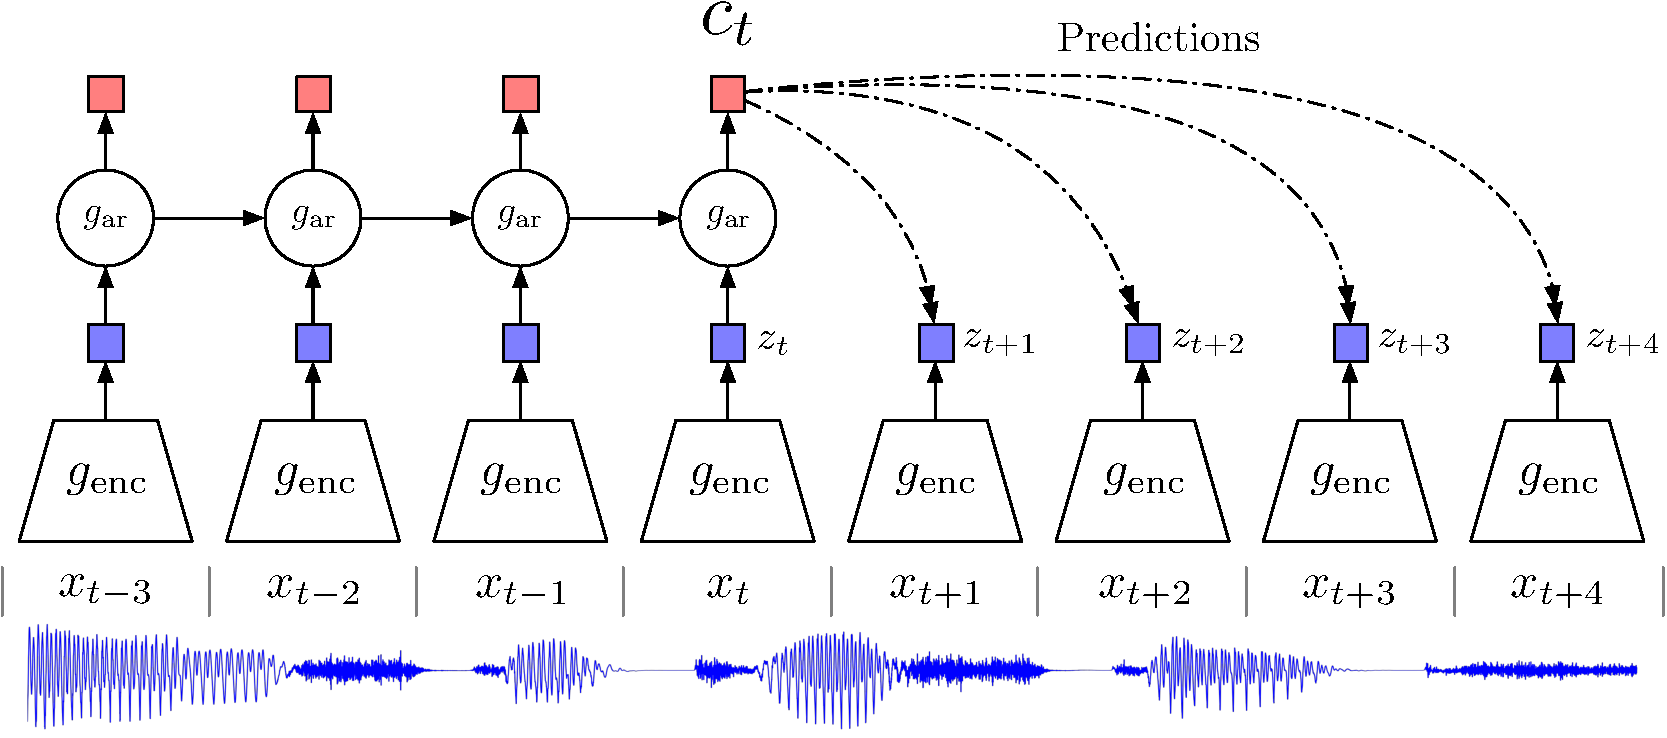
\includegraphics[width=0.9\textwidth]{images/CPC-paper-model.pdf}
	\caption{The Contrastive Predictive Coding model. Image from \cite{oord_representation_2019}}\label{fig:CPC-paper-model}
\end{figure}

\subsection{Application to MIL}

The core idea taken from CPC to clustering is that of the InfoNCE loss. The actual application is based on the following idea. If a bag is split into two parts, it is reasonable to expect that the representations of these two parts would be close to one another. On the other hand, if a random bag were to be drawn from the data (as a simple random sample with replacement), it is reasonable to expect it to be relatively far from any actual bag present in the data. Using these assumptions, the following clustering loss is constructed:

\[ B_k^{(1)} \oplus B_k^{(2)} = B_k \in \mathspace{B} \]
\[ B'_j = \mathrm{srswr} \left( \mathspace{X} \right) \]
\[ L_\mathrm{CPC} = \log \left\lVert \phi \left( B_k^{(1)} \right) - \phi \left( B_k^{(2)} \right) \right\rVert^2 - \log \sum_{j = 1}^K \left\lVert \phi \left( B_k^{(1)} \right) - \phi \left( B'_j \right) \right\rVert^2 \]
where \( \oplus \) is the multiset sum (see definition \ref{def:multiset-sum}). The first term of the loss function depicts the notion that the representations of the two parts of the bag should be close to one another. The second term depicts the notion that a random bag should be far from all the bags\footnote{On the off-chance a random bag would be close to \( B_k^{(1)} \), this would be outweighed by the other terms.}. The choice to use the first part of the bag in the second term has no effect as the two parts are chosen randomly. The value \( K \) is a hyper-parameter of this method.

This method can be further simplified. In order to not have to draw a lot of random bags, it can be reasonably expected that, on average, the representations of two parts of two mismatched bags \( B_{k_1}^{(1)} \) and \( B_{k_2}^{(2)} \) should be far apart. The matrix \( \mathmat{D} \) is constructed as
\[ \mathmat{D}_{ij} = \left\lVert \phi \left( B_i^{(1)} \right) - \phi \left( B_j^{(2)} \right) \right\rVert_2^2 \]
The distances of the corresponding halves are found on the diagonal of \( \mathmat{D} \), whereas the distances of mismatched halves are in the rest of the matrix. Under this assumptions the final loss for the CPC method is
\[ L_\mathrm{CPC} = \frac{1}{n} \sum_{i = 1}^n \left( \log \left( D_{ii} \right) - \log \sum_{\substack{j = 1 \\ j \neq i}}^n D_{ij} \right) \]
where \( n \) is the number of bags.
